

\section{Theoretische Grundlagen und Stand der Technik}

\subsection{Stand der Technik in der Objekterkennung}

Die moderne Objekterkennung wird heute maßgeblich von Deep-Learning-Ansätzen, insbesondere \textit{Convolutional Neural Networks} (CNNs), dominiert. Diese haben traditionelle Methoden, die auf handgefertigten Merkmalen wie HOG (\textit{Histogram of Oriented Gradients}) basierten, hinsichtlich Genauigkeit und Flexibilität weitgehend abgelöst. CNNs lernen Merkmale direkt aus den Daten und ermöglichen dadurch robustere und besser generalisierbare Modelle.

Innerhalb der Deep-Learning-basierten Objekterkennung existieren zwei Hauptstrategien:

\begin{enumerate}
    \item \textbf{Two-Stage Detectors:} Zunächst werden potenzielle Regionen (\textit{Region Proposals}) generiert, in denen sich Objekte befinden könnten. Anschließend werden diese Regionen klassifiziert (z.B. Faster R-CNN). Diese Ansätze erreichen oft eine hohe Genauigkeit, sind jedoch tendenziell langsamer.
    \item \textbf{One-Stage Detectors:} Hierbei wird die Objekterkennung als direktes Regressionsproblem formuliert. Bounding-Box-Koordinaten und Klassenwahrscheinlichkeiten werden in einem einzigen Durchlauf vorhergesagt. Bekannte Vertreter sind SSD (\textit{Single Shot MultiBox Detector}) und insbesondere YOLO (\textit{You Only Look Once}), die sich durch hohe Verarbeitungsgeschwindigkeit für Echtzeitanwendungen auszeichnen.
\end{enumerate}

\subsubsection{YOLO als Basis für schnelle Detektion}

YOLO unterteilt das Eingabebild in ein Gitter. Jede Zelle ist für die Erkennung von Objekten zuständig, deren Mittelpunkt in sie fällt. Für jede Zelle werden Begrenzungsrahmen, ein Konfidenzwert und Klassenwahrscheinlichkeiten vorhergesagt. 

Seit der ersten Veröffentlichung wurden zahlreiche Weiterentwicklungen (YOLOv3, v4, v5, \ldots, v8 etc.) vorgestellt, die:
\begin{itemize}
    \item die Architektur verfeinerten,
    \item die Genauigkeit, insbesondere bei kleinen Objekten, verbesserten und
    \item Techniken wie Feature Pyramid Networks zur besseren Merkmalsextraktion integrierten.
\end{itemize}

Die Stärke von YOLO liegt in seiner Geschwindigkeit. Daher eignet es sich besonders für die initiale Detektion von Objekten wie Gesichtern oder Kennzeichen in Videoströmen, wie auch in diesem Projekt genutzt.

\subsubsection{MediaPipe für detaillierte Wahrnehmung auf Endgeräten}

Parallel zur Entwicklung von Detektionsarchitekturen wie YOLO gewinnen Frameworks wie Google's MediaPipe an Bedeutung. MediaPipe bietet optimierte, vortrainierte Modelle und komplette, plattformübergreifende Pipelines für spezifische Wahrnehmungsaufgaben direkt auf Endgeräten (Mobilgeräte, Web). 

Es spezialisiert sich auf die effiziente Extraktion detaillierter Informationen, wie:
\begin{itemize}
    \item hochauflösende Gesichtsgitter (\textit{Face Mesh}),
    \item Hand- oder Körper-Landmarken,
\end{itemize}
und ermöglicht damit Anwendungen wie Gestensteuerung, AR-Effekte oder die Analyse biometrischer Merkmale in Echtzeit.

\subsubsection{Kombination von Ansätzen}

Häufig werden verschiedene Ansätze kombiniert. Ein schneller Detektor wie YOLO kann die grobe Position eines Gesichts bestimmen. Anschließend extrahieren spezialisierte Modelle wie MediaPipe detaillierte Landmarken innerhalb der detektierten Region. Dieser hybride Ansatz vereint Geschwindigkeit und Detailgenauigkeit.

Für die Anforderungen dieses Projekts – schnelle und zuverlässige Erkennung von Kennzeichen und Gesichtern sowie die detaillierte Analyse von Gesichtsmerkmalen – sind sowohl die YOLO-Architektur als auch das MediaPipe-Framework relevante Technologien.

\subsection{Funktionsweise von YOLO}

YOLO (\textit{You Only Look Once}) verfolgt einen effizienten Ansatz für die Objekterkennung, der sich durch seine hohe Geschwindigkeit auszeichnet. Anstatt das Bild in mehreren Schritten zu analysieren, betrachtet YOLO das gesamte Bild nur einmal (daher der Name) und sagt alle Objekte gleichzeitig vorher. Man kann sich das wie ein schnelles „Überfliegen“ des Bildes vorstellen.

\begin{figure}[htbp]
    \centering
    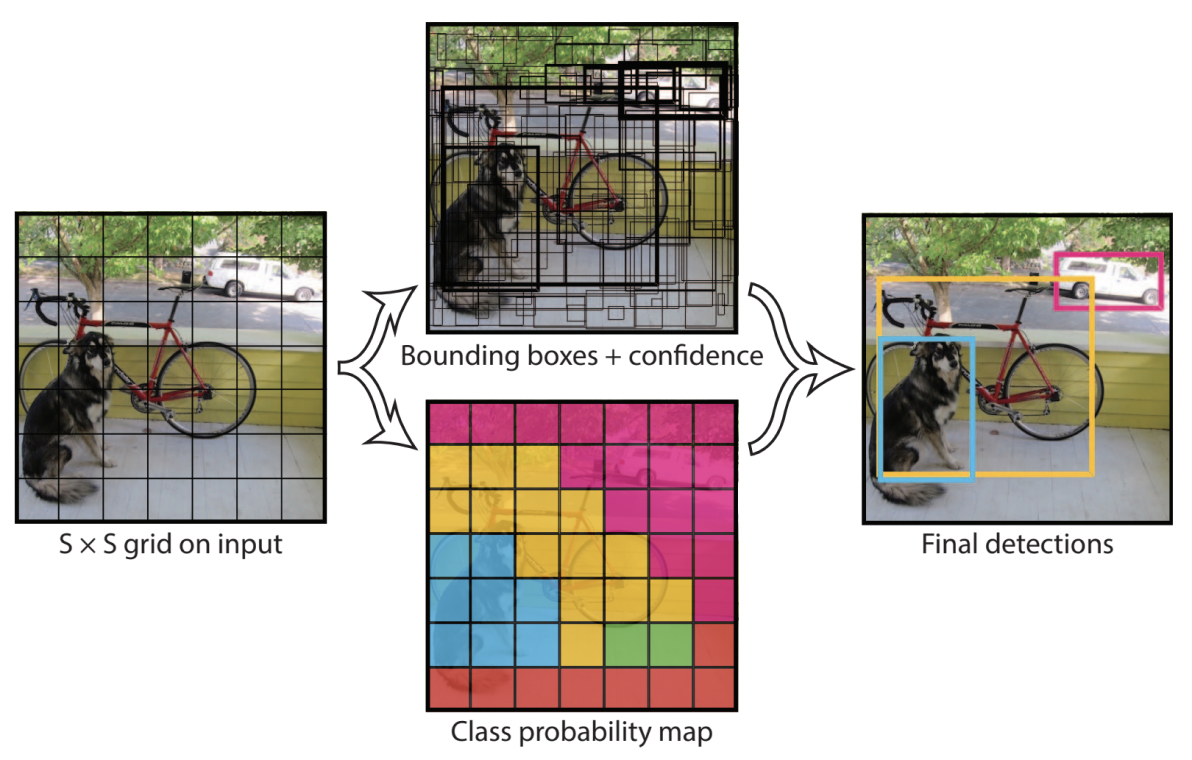
\includegraphics[width=0.8\textwidth]{data/yolo_grid.png}
    \caption{YOLO-Architektur: Das Bild wird in ein Gitter unterteilt, jede Zelle sagt Bounding Boxes und Klassenwahrscheinlichkeiten voraus. Quelle: \cite{yolo_grid}}
    \label{fig:yolo_grid}
\end{figure}

\textbf{Das Gitter (Grid):} \\
Der Kern von YOLO ist die Aufteilung des Eingangsbildes in ein gedachtes Gitter, ähnlich einem Schachbrett (z.B. $13 \times 13$ oder $19 \times 19$ Zellen). Jede dieser Zellen bekommt eine spezielle Aufgabe: Sie ist dafür verantwortlich, Objekte zu erkennen, deren Mittelpunkt genau in diese Zelle fällt.

\textbf{Vorhersagen pro Zelle:} \\
Jede Zelle im Gitter macht mithilfe eines neuronalen Netzes Vorhersagen über mögliche Objekte:
\begin{itemize}
    \item \textbf{Bounding Boxes:} Die Zelle schlägt eine oder mehrere „Boxen“ (Rechtecke) vor, die ein Objekt umschließen könnten. Für jede Box werden Position (x-, y-Koordinaten des Mittelpunkts), Größe (Breite $w$, Höhe $h$) und ein Konfidenzwert vorhergesagt. Dieser Konfidenzwert gibt an, wie sicher sich das Modell ist, dass sich überhaupt ein Objekt in der Box befindet und wie gut die Box passt.
    \item \textbf{Klassenwahrscheinlichkeiten:} Zusätzlich sagt die Zelle voraus, zu welcher Klasse (z.B. „Auto“, „Person“, „Kennzeichen“) ein erkanntes Objekt am wahrscheinlichsten gehört.
\end{itemize}

\textbf{Architektur und Entwicklung:} \\
Das Herzstück ist ein einzelnes Convolutional Neural Network (CNN), das diese Vorhersagen für alle Zellen gleichzeitig generiert. Frühe Versionen nutzten Architekturen wie Darknet. Spätere Versionen (YOLOv3 bis YOLOv8) wurden deutlich komplexer und leistungsfähiger, indem sie z.B. Merkmale aus verschiedenen Ebenen des Netzwerks kombinieren (Feature Pyramid Networks, FPN), um sowohl kleine als auch große Objekte besser zu erkennen. Auch wurden \textit{Anchor Boxes} eingeführt – vordefinierte Box-Formen, die dem Netzwerk helfen, Objekte mit typischen Seitenverhältnissen schneller und genauer zu finden.

\textbf{Aufräumen der Ergebnisse (Non-Max Suppression, NMS):} \\
Da oft mehrere Zellen oder Boxen dasselbe Objekt erkennen, liefert YOLO zunächst viele überlappende Boxen. Um nur die relevanteste Box pro Objekt zu behalten, wird ein „Aufräumschritt“ namens Non-Max Suppression (NMS) durchgeführt. Dabei werden Boxen mit geringer Konfidenz entfernt und von den verbleibenden, überlappenden Boxen wird nur die mit der höchsten Konfidenz behalten, während die anderen verworfen werden.

\textbf{Versionen:} \\
YOLO wird ständig weiterentwickelt. In diesem Projekt kam hauptsächlich YOLOv8 zum Einsatz. Diese Version stellt einen aktuellen Stand der Technik dar und bietet eine gute Balance aus Erkennungsgenauigkeit und hoher Geschwindigkeit, was für die Analyse von Videoströmen vorteilhaft ist. Sie profitiert von den Architekturoptimierungen und Trainingstechniken früherer Versionen und ist oft einfacher zu verwenden. Die Entwicklung schreitet kontinuierlich voran, wie neuere, von Ultralytics dokumentierte Varianten wie YOLOv11 zeigen, was die Dynamik in diesem Bereich unterstreicht.

\subsection{OCR für Texterkennung}

\subsection{Gesichtserkennung mit neuronalen Netzen}